%% Condensed from dissertacao-en/chapters/cap7-destilacao.tex @295dde3.
%% Every number and qualifier exists in the extended report (same chapter).
\chapter{Distributional Distillation}
\label{chap:destilacao}

The benchmark's accuracy leader costs four to five orders of
magnitude more latency per row than a gradient-boosted tree. This
chapter asks what of a tabular foundation model's advantage can be
carried into a student that serves fast --- and answers RQ3 with a
selective result: \emph{point} distillation does not transfer,
\emph{distributional} distillation transfers a modest, measurable
part, and the conditions under which it is worth doing can be
checked before training the student. Full process record, ablation
tables and per-run artifacts are in the extended technical report
and in the project repository.

\section{Question and setup}
\label{sec:destil-setup}

\textbf{Teacher.} TabPFN-2.5 \citep{hollmann2025,priorlabs2025}, an
8-member ensemble with the training context capped at 50{,}000 rows,
re-labels each dataset's training pool \emph{out-of-fold} (OOF): the
pool is split into folds, and each fold receives predictions from a
teacher whose context excludes it. The teacher natively outputs a
predictive distribution, read as 19 quantile curves
($\tau \in \{0.05, \ldots, 0.95\}$). TabFM cannot play this role:
its regression head is point-valued (an architectural negative
confirmed by the official technical report, \citealp{kong2026});
Section~\ref{sec:destil-ponto} uses it as a point-teacher anchor.

\textbf{Students and control.} The distilled student is the
benchmark's XGBoost with a 19-output head trained by squared error
on the teacher's quantile curves; the \emph{control} is the same
architecture trained by pinball loss on the true labels --- so the
teacher is the only difference between the arms. A point student
(single output, trained on the teacher's means) answers H1, and a
true-label quantile MLP enters the decision rule's analysis. All
students inherit the benchmark's tuned hyperparameters; the
re-tuning analysis below removes that crutch.
Figure~\ref{fig:destil-pipeline} summarizes the pipeline.

\begin{figure}[htb]
\centering
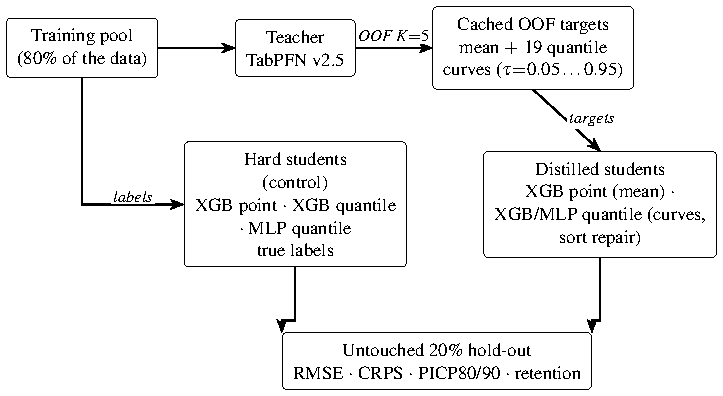
\includegraphics{images/tikz-cap7-1-en.pdf}
\caption[Distributional distillation pipeline]{Distributional
distillation pipeline: the teacher labels the pool OOF with 19
quantile curves; the distilled student regresses on the curves; the
control learns the same quantiles from the true labels. Source: the
author.}
\label{fig:destil-pipeline}
\end{figure}

\textbf{Metric.} Quality is CRPS on the untouched hold-out,
estimated from the 19 quantiles. The headline quantity is
\emph{retention}: the fraction of the teacher's CRPS advantage over
the control that the distilled student preserves,
$(\mathrm{CRPS}_{\mathrm{ctrl}} -
\mathrm{CRPS}_{\mathrm{dist}})/(\mathrm{CRPS}_{\mathrm{ctrl}} -
\mathrm{CRPS}_{\mathrm{teach}})$. On \texttt{cpu\_activity}, for
example, the control scores 1.294, the teacher 1.061 and the
distilled student 1.178: the student recovers half of the gap
(retention $+0.500$), a 9.0\% CRPS gain over the control.

\textbf{Datasets.} 20 regression datasets: the 5 central ones plus
15 from the OpenML-CTR23 suite. Four eligible CTR23 datasets were
left out of the extension (one with no recorded justification); a
sensitivity run on five data splits puts the scoreboard with them at
17/24 ($p=0.032$), and excluding the two datasets that overlap the
teacher's pre-training corpus gives 16/22 ($p=0.026$) --- the
verdict does not depend on the roster choice.

\section{Registered design}
\label{sec:destil-desenho}

The design was registered in two stages: the July~15 pre-registration
fixed H1--H3 on the five central datasets before any execution; the
confirmatory sign test and the extension's eligibility rule were
fixed at an interim reading (11/15, $p=0.059$), and the final test
therefore carries a two-stage sequential correction --- the headline
$p=0.006$ is reported as $p\approx0.019$ after splitting the
significance level across the two looks (single-stage threshold
0.0118). Table~\ref{tab:destil-hipoteses} lists every hypothesis and
analysis with its registration status and verdict; negative results
are reported with the same prominence as positive ones.

\begin{table}[htb]
\centering
\caption[The chapter's hypotheses and registration status]{The
chapter's hypotheses and analyses: what each claims, whether it was
fixed before any reading of results, and the verdict. Dates and full
records in the extended report.}
\label{tab:destil-hipoteses}
\small
\begin{tabular}{>{\raggedright\arraybackslash}p{0.14\linewidth}>{\raggedright\arraybackslash}p{0.35\linewidth}>{\raggedright\arraybackslash}p{0.18\linewidth}>{\raggedright\arraybackslash}p{0.21\linewidth}}
\toprule
Code & What it claims & Before reading? & Verdict \\
\midrule
H1 (point) & point student retains $\geq$50\% of the RMSE gap on
$\geq$3/5 & yes & refuted (0/5 central datasets reach 50\%
retention; descriptively, it beats the control on 4/20) \\
\addlinespace[2pt]
H2 (distribution) & distilled beats the control in CRPS, with
coverage within $\pm$5~p.p. & yes & not confirmed as a conjunction:
CRPS clause sustained (16/20); coverage clause not met (10/20) \\
\addlinespace[2pt]
H3 (Pareto) & there is a latency band where the distilled student
dominates the compressed teacher & yes & not confirmed as
registered: dominance only on \texttt{year}, at 169~\us{} (above
the ${\lesssim}100$ band); within the band, merely non-dominated,
and only on california$^\dagger$; refuted on \texttt{kin8nm} \\
\addlinespace[2pt]
Sign test & confirmatory instrument of the 16/20 & no (fixed at the
interim reading) & $p\approx0.019$ sequential \\
\addlinespace[2pt]
Heavy tail (log) & redoing teacher and students with
$y'{=}\log(1{+}y)$ recovers retention on the price-scale failures &
no (fixed at the interim reading, before the ablation) & refuted
(\texttt{fifa} goes from $-1.29$ to $-1.69$ in the transformed
space; the two controls move in opposite directions) \\
\addlinespace[2pt]
E1 (classical) & distilled beats the best of QRF and NGBoost & yes
(execution already started) & confirmed (17/20) \\
\addlinespace[2pt]
E3 (utility) & realized cost lower or equal at $\tau{=}0.90$ &
registered (before any reading) & confirmed (18/20) \\
\addlinespace[2pt]
Re-tuning & inherited hyperparameters are a floor on retention &
partially (pilot read before; extension to the 20 registered in a
dated addendum) & refuted (9/20 per dataset; median
0.19$\to$0.12): sign upheld, magnitude reduced \\
\bottomrule
\end{tabular}
\end{table}

\section{Point distillation does not transfer}
\label{sec:destil-ponto}

The first result is the negative the pre-registration committed to
report. Across the 20 datasets, the point student trained on the
teacher's means beats its true-label control on only \textbf{4}; H1
is refuted already on the five central datasets (0/5 reach the
registered 50\% retention). The natural objection --- ``the teacher
was not strong enough'' --- was tested directly by replicating the
experiment with TabFM as teacher on the five central datasets: its
reference advantage is almost $6\times$ TabPFN's on
\texttt{california\_\allowbreak housing}$^\dagger$ (0.028 against
0.005 RMSE), and the negative holds --- with the caveat that this
anchor rests on a single, binarized-target dataset. A pool-size
sweep (caps 800/2{,}000/8{,}000) shows a genuine low-data gain only
on \texttt{wine\_quality} ($\Delta=+0.026$ at $n{=}800$), gone from
$n{=}2{,}000$ on, and on california$^\dagger$ only a marginal
$+0.005$ residue at 2{,}000. At realistic pool sizes, what the
teacher knows about the \emph{mean}, a tuned GBDT learns on its own
from the raw labels.

\section{Distributional distillation transfers part of the advantage}
\label{sec:destil-dist}

The distilled quantile student beats its control in CRPS on
\textbf{16 of 20} datasets (sign test $p=0.006$ single-stage,
$p\approx0.019$ under the sequential correction), with median
retention $+0.19$ and a median CRPS gain of 2.8\% over the control.
Table~\ref{tab:destil-retencao} gives the result per dataset and
Figure~\ref{fig:destil-forest} the same picture with uncertainty:
by bootstrap confidence interval the scoreboard is 12 clear wins, 1
win at the margin, 3 ties with a positive point estimate, 1 tie with
a negative one, and 3 clear defeats. Two supplementary instruments
agree with different firmness: one-sided Wilcoxon $p=0.045$
(two-sided 0.090 would not reject), and the Bayesian signed-rank
analysis assigns probability 0.96 that the positive-retention region
is the most probable one (ROPE $\pm0.05$; expected posterior mass on
it: $E[\theta]=0.70$).

\begin{table}[htb]
\centering
\caption[Distributional distillation result per dataset]{Result per
dataset (mean of 3 seeds), sorted by retention. Gain = relative CRPS
reduction over the control; CI by bootstrap over hold-out rows.
$^\dagger$binarized-target erratum dataset.}
\label{tab:destil-retencao}
\scriptsize
\setlength{\tabcolsep}{4pt}
\begin{tabular}{lrrrrrr}
\toprule
Dataset & CRPS ctrl & CRPS dist & CRPS teach & Gain (\%) & 95\% CI (\%) & Retention \\
\midrule
pumadyn32nh & 0.0130 & 0.0124 & 0.0124 & $+$4.7 & [3.7; 5.7] & $+$1.057 \\
california\_housing$^\dagger$ & 0.1802 & 0.1086 & 0.0691 & $+$39.7 & [37.1; 42.3] & $+$0.644 \\
abalone & 1.154 & 1.098 & 1.060 & $+$4.9 & [3.0; 6.7] & $+$0.595 \\
fps\_benchmark & 0.4651 & 0.3855 & 0.3128 & $+$17.1 & [15.1; 19.0] & $+$0.523 \\
cpu\_activity & 1.294 & 1.178 & 1.061 & $+$9.0 & [6.4; 11.6] & $+$0.500 \\
cps88wages & 160.8 & 160.6 & 160.4 & $+$0.1 & [$-$0.1; 0.3] & $+$0.465 \\
year\_prediction & 4.558 & 4.427 & 4.246 & $+$2.9 & [2.6; 3.2] & $+$0.419 \\
online\_news & 0.4554 & 0.4540 & 0.4497 & $+$0.3 & [0.0; 0.6] & $+$0.255 \\
sarcos & 1.270 & 1.163 & 0.7961 & $+$8.4 & [7.4; 9.4] & $+$0.225 \\
kings\_county & 50{,}516 & 48{,}969 & 43{,}262 & $+$3.1 & [1.5; 4.6] & $+$0.213 \\
grid\_stability & 0.0043 & 0.0038 & 0.0017 & $+$10.3 & [8.6; 12.0] & $+$0.170 \\
kin8nm & 0.0682 & 0.0644 & 0.0380 & $+$5.7 & [4.4; 7.0] & $+$0.128 \\
physiochemical\_protein & 1.785 & 1.736 & 1.212 & $+$2.8 & [1.9; 3.6] & $+$0.086 \\
video\_transcoding & 0.3053 & 0.2974 & 0.2138 & $+$2.6 & [0.1; 5.0] & $+$0.086 \\
space\_ga & 0.0601 & 0.0592 & 0.0488 & $+$1.5 & [$-$0.9; 3.8] & $+$0.078 \\
miami\_housing & 31{,}999 & 31{,}931 & 27{,}882 & $+$0.2 & [$-$1.9; 2.3] & $+$0.016 \\
health\_insurance & 7.273 & 7.311 & 7.122 & $-$0.5 & [$-$1.3; 0.2] & $-$0.255 \\
diamonds\_real & 192.5 & 195.5 & 183.1 & $-$1.5 & [$-$2.4; $-$0.6] & $-$0.315 \\
wine\_quality & 0.3277 & 0.3652 & 0.2891 & $-$11.4 & [$-$14.6; $-$8.5] & $-$0.970 \\
fifa & 2{,}837 & 2{,}893 & 2{,}795 & $-$1.9 & [$-$3.8; $-$0.1] & $-$1.287 \\
\bottomrule
\end{tabular}
\end{table}

\begin{figure}[htb]
\centering
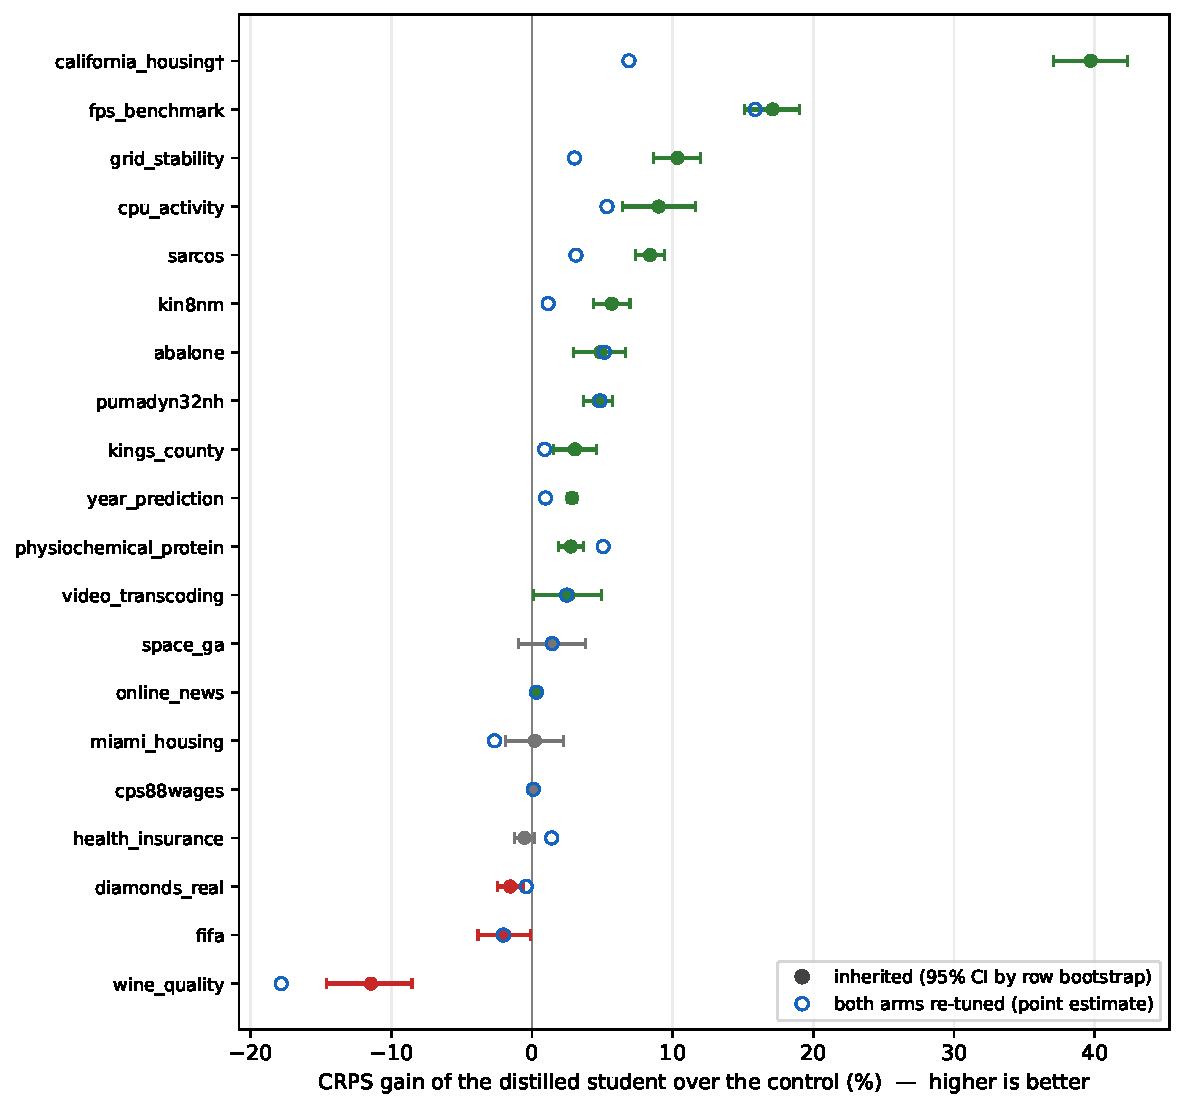
\includegraphics[width=0.92\linewidth]{images/forest_distill_en.pdf}
\caption[CRPS gain per dataset, with uncertainty]{Relative CRPS gain
of the distilled student over the control, with bootstrap 95\% CIs
(log-scaled axis). Source:
\texttt{results/distillation}.}
\label{fig:destil-forest}
\end{figure}

\textbf{Re-tuning: the honest magnitude.} The inherited
hyperparameters were searched for squared error --- the distilled
arm's loss, not the control's. Re-tuning both arms separately
(Optuna, 25 trials each) does not change the scoreboard (16/20,
$p=0.006$; without the binarized dataset 15/19, $p=0.010$) but
halves the magnitude: median retention 0.19$\to$0.12, median CRPS
gain 2.8\%$\to$1.4\% (the re-tuned mean retention is $-0.02$, pulled
by the negatives). The number this work stands behind is therefore a
median CRPS gain of 1.4--2.8\% (retention of 12--19\% of the
teacher's advantage), with the lower end as the conservative
estimate. Table~\ref{tab:destil-robustez} gathers all the
robustness variants.

\begin{table}[htb]
\centering
\caption[Robustness of the distributional distillation verdict]{The
verdict under every variation: roster, re-tuning, seeds and splits.}
\label{tab:destil-robustez}
\small
\setlength{\tabcolsep}{3pt}
\begin{tabular}{lcccc}
\toprule
Variant & Score & Median ret. & Sign (one-s.) & Wilcoxon (one-s.) \\
\midrule
Main (inherited, 3 seeds) & 16/20 & 0.19 & 0.006 (0.019 seq.) & 0.045 \\
Without the binarized & 15/19 & 0.17 & 0.010 & 0.067 \\
Both arms re-tuned & 16/20 & 0.12 & 0.006 & 0.035 \\
Re-tuned, without the binarized & 15/19 & 0.10 & 0.010 & 0.048 \\
Ten student seeds & 16/20 & 0.19 & --- & --- \\
With the 4 omitted eligible (5 splits) & 17/24 & --- & 0.032 & --- \\
Without the 2 overlapping the core (5 splits) & 16/22 & --- & 0.026 & --- \\
\bottomrule
\end{tabular}
\end{table}

\textbf{The defeats are diagnosable.} \texttt{wine\_quality} is a
dataset artifact: 27.6\% of the test set has an exact covariate twin
in the pool (1{,}179 duplicated rows), and on the deduplicated
dataset ($n=5{,}318$, teacher re-labeled OOF) the defeat disappears.
\texttt{health\_\allowbreak insurance} is configuration-sensitive,
not structural: its retention goes from $-0.26$ (inherited) to
$+0.65$ (re-tuned). \texttt{fifa} and
\texttt{diamonds\_\allowbreak real} remain unexplained failures on
price-scale targets --- and the registered heavy-tail hypothesis
(that a $\log(1{+}y)$ re-run would rescue them) was refuted:
\texttt{fifa} goes from $-1.29$ to $-1.69$ in the transformed space,
and the two positive controls move in opposite directions.

\textbf{Coverage: the H2 clause that fails.} The distilled student's
central-interval coverage lands within $\pm5$~p.p.\ of nominal on
only 10 of 20 datasets (2/5 core), so H2 is not confirmed as a
conjunction: the CRPS clause holds (16/20), the coverage clause does
not. Calibration is the dimension to watch, and
Section~\ref{sec:destil-oof} shows where it comes from.

\section{The serving frontier}
\label{sec:destil-fronteira}

To answer H3, accuracy and latency of \emph{all} strategies ---
distill, compress the teacher's context, shrink its ensemble ---
were measured on the same hold-outs of three positive-advantage
datasets (Figure~\ref{fig:destil-pareto}). The distilled student
delivers CRPS 0.109 at 99~\us/row where the teacher's cheapest
configuration needs 245~\us/row for 0.094
(california$^\dagger$), and 4.43 at 169~\us/row where the cheapest
teacher that beats it costs 4{,}576~\us/row ($27\times$ the latency)
on \texttt{year\_\allowbreak prediction}. On \texttt{kin8nm} the
picture inverts, instructively: the teacher's absolute advantage is
small ($+0.030$ CRPS; its relative advantage, 44\%, is among the
largest) and a \emph{single-member} TabPFN delivers CRPS 0.040 at
150~\us/row --- essentially the student's latency --- so ensemble
shrinking, not distillation, is the right lever: a latency case, not
a small-advantage case.

H3's verdict: \textbf{not confirmed as registered}. Pareto dominance
over the subsampled teacher occurs only on
\texttt{year\_\allowbreak prediction}, at 169~\us/row --- above the
pre-registered ${\lesssim}100$~\us/row band; within the band the
student is merely \emph{non-dominated} (no teacher configuration
operates below 245~\us) and only on california$^\dagger$, where its
CRPS is 15.5\% worse than the teacher's cheapest configuration;
without the binarized dataset the band is not met at all; on
\texttt{kin8nm} the hypothesis is refuted. What stands is the
latency reading: where no cheap teacher configuration reaches the
student's tier, the distilled student is the CRPS-optimal
teacher-derived system in that regime. A side finding: shrinking
TabPFN from 8 members to 1 \emph{improved} RMSE on
california$^\dagger$ (0.2521 against 0.2555) at a seventh of the
latency --- ensemble shrinking is an underrated first lever.

\begin{figure}[htb]
\centering
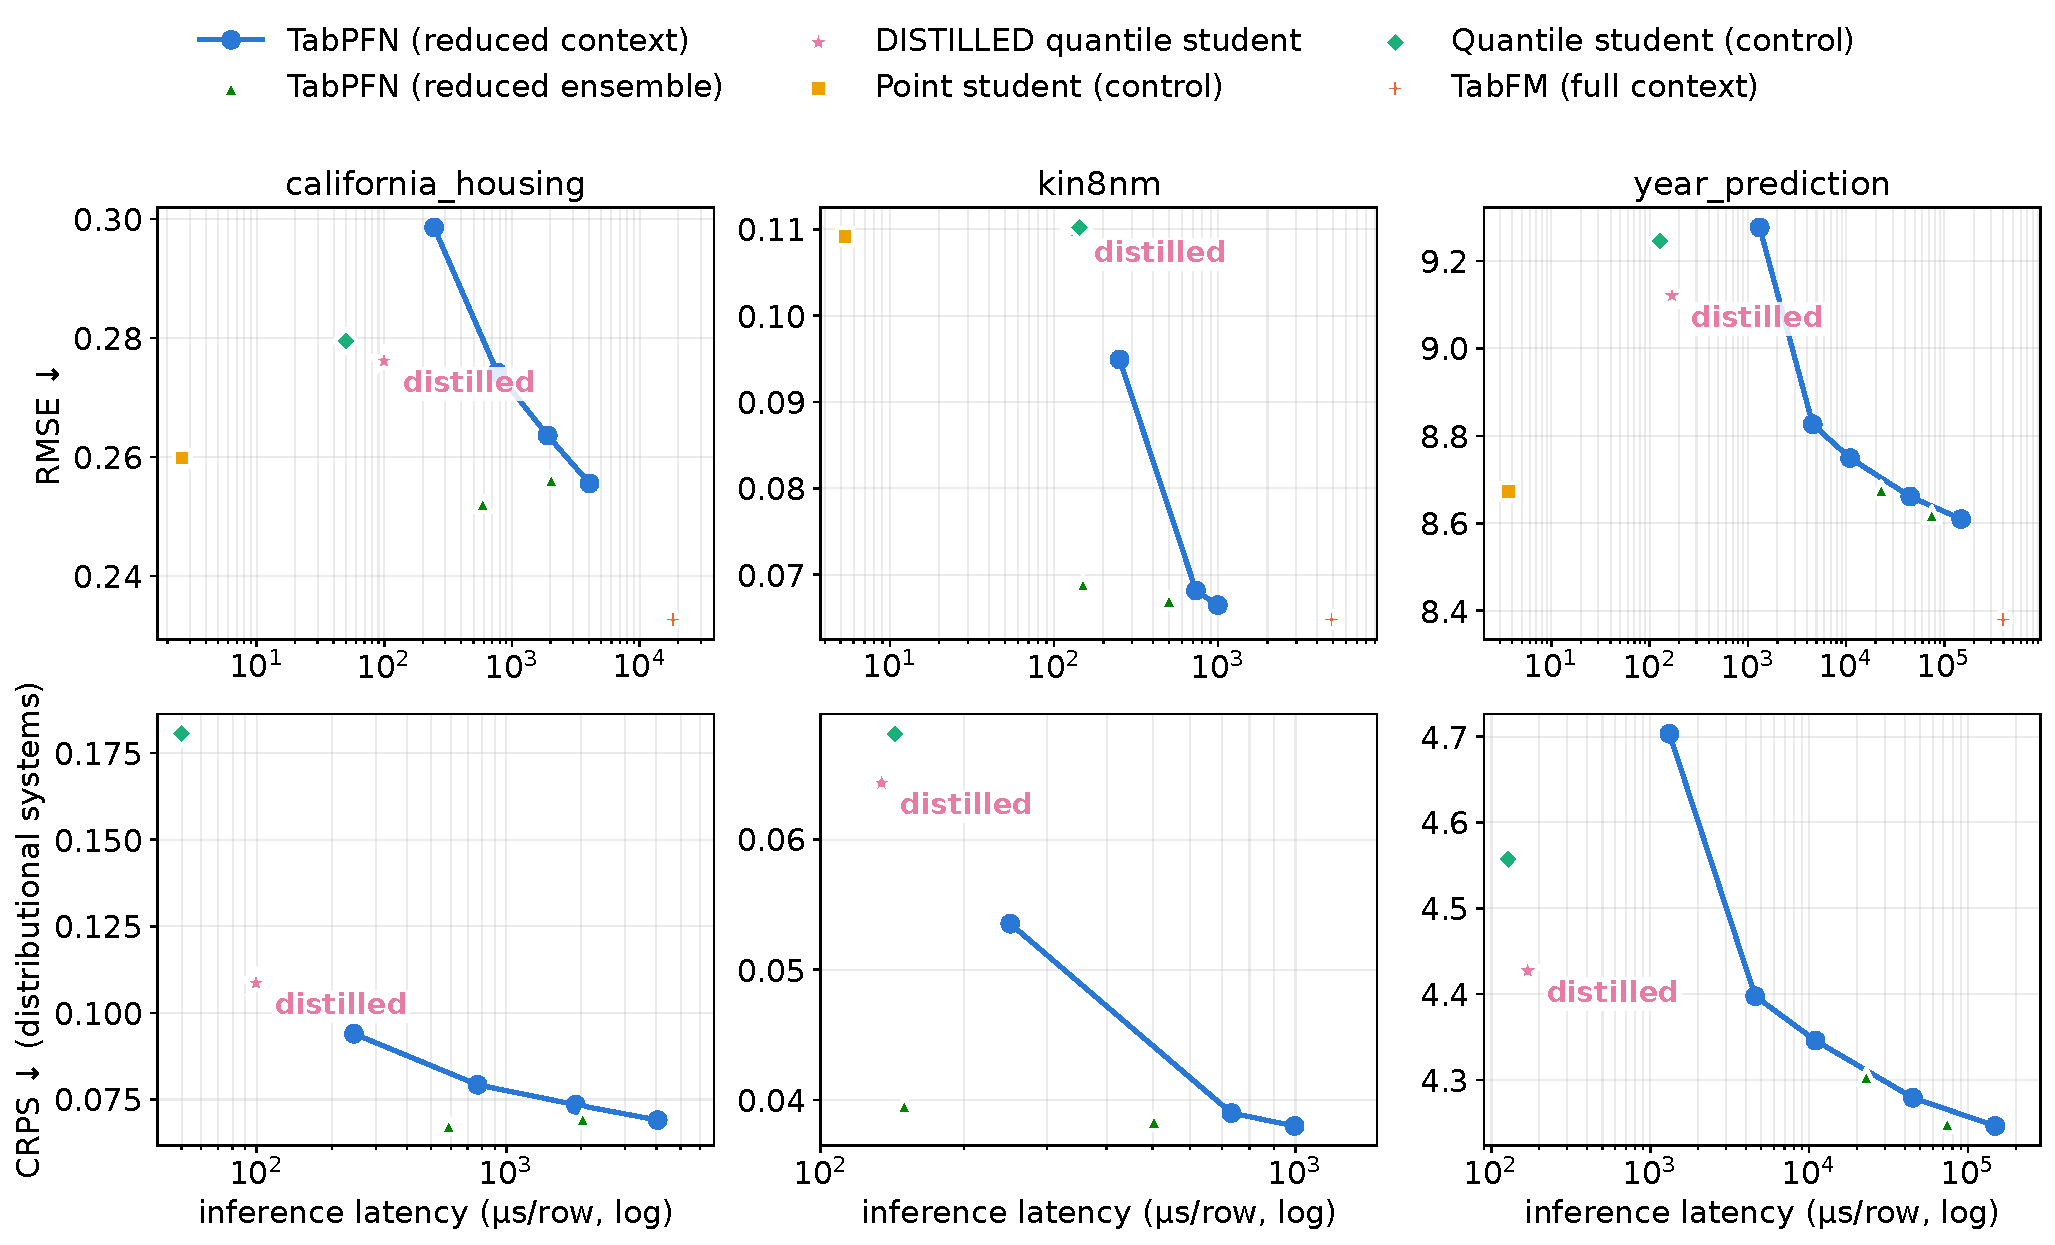
\includegraphics[width=\linewidth]{images/pareto_distill_en.pdf}
\caption[Frontier distill $\times$ compress $\times$ shrink]{The
serving frontier on three datasets: RMSE (top) and CRPS (bottom)
against latency (log). The teacher's context-compression curve, its
shrunk-ensemble points, the distilled student and the controls, with
TabFM (full context) as the accuracy anchor. Source:
\texttt{results/distillation/pareto.csv}.}
\label{fig:destil-pareto}
\end{figure}

\section{OOF labeling protects calibration, not accuracy}
\label{sec:destil-oof}

An ablation relabeling the pool \emph{in-sample} (teacher sees the
rows it labels) moves CRPS by at most ${\sim}0.003$ on three of four
datasets --- and on \texttt{wine\_quality} the in-sample run
\emph{improves} CRPS by 0.029, consistent with the
duplicate-memorization mechanism above. What leakage degrades is
\emph{calibration}: OOF labeling keeps the student's central-interval
coverage 0.5--5.1~p.p.\ closer to nominal. OOF labeling is therefore
the student's calibration safeguard, not an accuracy booster.
Figure~\ref{fig:destil-calibration} shows the hold-out reliability
curves; the reading rule, corrected mid-study, is that the
\emph{slope} decides (steeper than the diagonal = overcoverage) ---
there is no shortcut ``above the diagonal = overcovers''. Two
post-hoc repairs are measured in the extended report: re-sorting the
19 quantile curves repairs 96\% of the crossing violations, and
split-conformal calibration fixes both arms' coverage while leaving
CRPS essentially intact --- distillation and conformalization are
complementary.

\begin{figure}[htb]
\centering
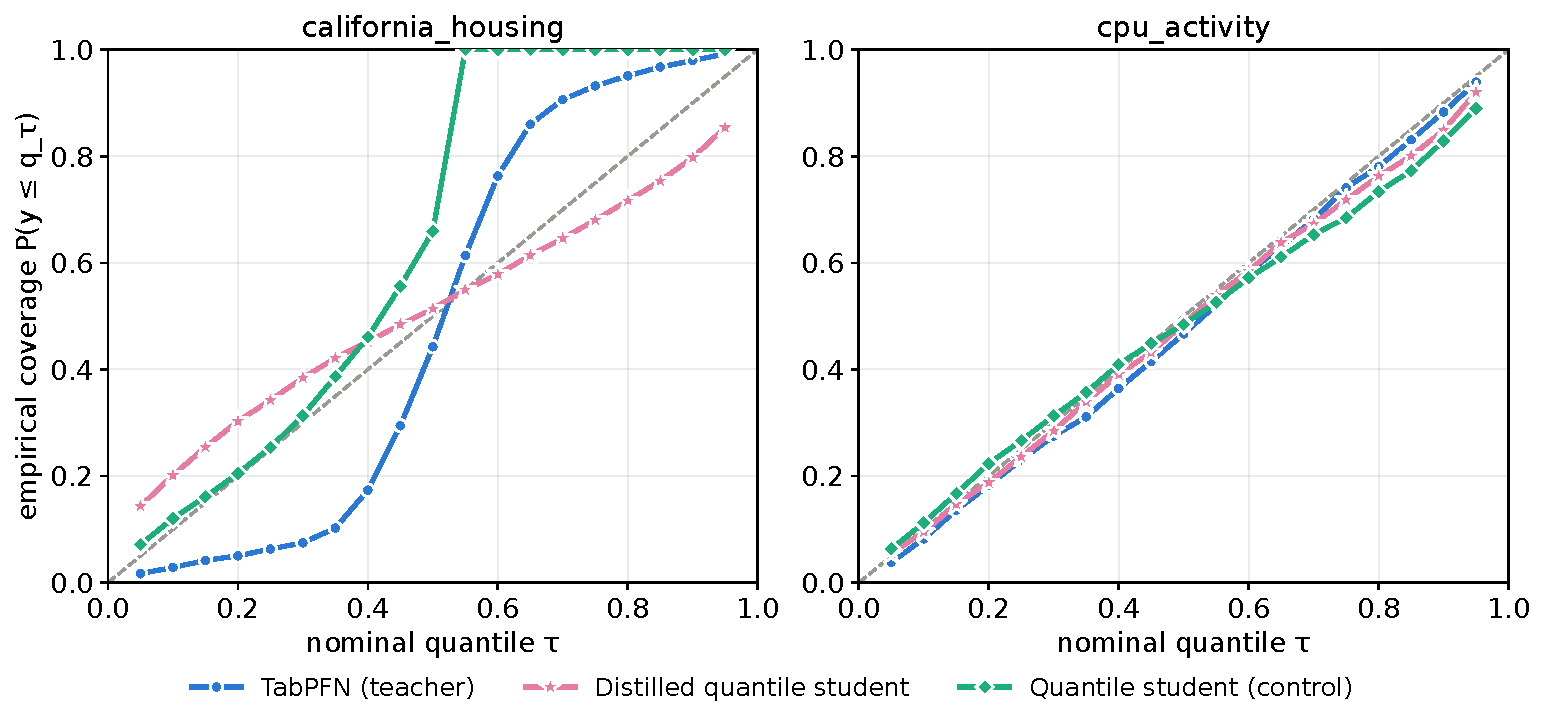
\includegraphics[width=0.9\linewidth]{images/calibration_distill_en.pdf}
\caption[Reliability on the hold-out]{Reliability curves on the
hold-out: empirical coverage $P(y \le q_\tau)$ against nominal
$\tau$, for teacher, distilled student and control, on the
binarized-target california$^\dagger$ (a Bernoulli calibration) and
on \texttt{cpu\_activity}, where the three systems are well
calibrated. Source: \texttt{results/distillation}.}
\label{fig:destil-calibration}
\end{figure}

\section{Classical distributional baselines (E1)}
\label{sec:destil-e1}

Registered question: does the distilled student beat strong
classical baselines that need no teacher at all? Against the best of
Quantile Regression Forest and NGBoost in \emph{default}
configuration, the distilled student wins in CRPS on \textbf{17 of
20} datasets (one-sided sign test $p=0.0013$); against the best
teacher-free alternative chosen \emph{per dataset} by an oracle
(QRF, NGBoost, quantile MLP, or a Gaussian point-plus-residual
baseline), 12 of 20 ($p=0.25$) --- distillation's edge over a
well-chosen native is real but not statistically separable. The
three upsets are diagnosable: on \texttt{wine\_quality} --- flagged
in advance by the registered eligibility criterion --- the default
QRF beats even the teacher; on california$^\dagger$ the QRF (CRPS
0.084) occupies the student's latency band with a better score; on
\texttt{physiochemical\_\allowbreak protein} the teacher's advantage
is thin. The QRF serves at 4.1--21.4~\us/row and NGBoost at
12.2--31.9~\us/row: the classical baselines live in the student's
latency regime, which is exactly why the decision rule makes
``test a strong native first'' a mandatory step.

\section{Decision utility (E3)}
\label{sec:destil-e3}

Registered before any reading: in a newsvendor-style reserve task at
$\tau=0.90$, provisioning by the distilled student's quantile yields
realized cost lower than or equal to the control's on \textbf{18 of
20} datasets ($p=0.0002$; by the conservative reading, 17/19
$p=0.0004$). The pre-declared exploratory profile explains why the
gain matters where it matters: the cost reduction is ${\sim}1\%$ at
central quantiles and rises to ${\sim}8\%$ in the tails --- e.g.\ on
\texttt{fps\_benchmark} the distilled reserve costs 103 against the
control's 108 per decision. Distributional quality translates into
money exactly where point predictions fail.

\section{When to distill: the decision rule}
\label{sec:destil-regra}

The rule condenses four results of the chapter --- the refuted point
and heavy-tail hypotheses, E1's upsets and the serving frontier:

\begin{quote}
\textbf{Before distilling: (i)~run cheap target transformations as a
diagnostic (a log on price-scale targets is free and changes the
error regime; in the ablation its directional effect is mixed and
marginal --- not a rescue); (ii)~test a strong native distributional
student --- a default QRF costs seconds, a quantile MLP covers the
small, numeric datasets. Distill when a genuine teacher advantage
persists after both --- a single OOF labeling measures that
advantage directly, at a cost of minutes to a few hours depending on
pool size and teacher latency. Where no cheap teacher configuration
reaches the student's latency tier, distillation is the
teacher-derived strategy that carries part of the advantage below
the teacher's cheapest competitive configuration (a strong native
QRF occupies the same latency regime and beats the distilled student
on 3 of 20 datasets); where a single teacher member already runs at
the student's latency, ensemble shrinking may settle the matter.}
\end{quote}

Two honesty notes bound the rule's status: its advantage gate was
verified in the \emph{oracle} version (the OOF version, the one a
practitioner would use, was not evaluated), and the rule was derived
on the same 20 datasets --- there is no out-of-sample test of the
rule itself.

\section{Limitations and synthesis}
\label{sec:destil-limitacoes}

The design inherits the benchmark's non-nested protocol; the teacher
is a single model (TabPFN-2.5) and the scope is regression only,
with TabFM's spread checked on a single, binarized-target dataset;
students inherit benchmark hyperparameters, and the re-tuning
analysis shows the inherited setting \emph{overstates} the
magnitude (0.19$\to$0.12). No multiplicity correction is applied
across experiments; under Holm at the 5\% level over the three main
sign tests the conclusions stand (adjusted $p \approx 0.019$;
$0.0026$; $0.0006$), the supplementary instruments do not, and in a
family including them the headline's adjusted $p$ would be 0.057.
The Bayesian 0.96 is the probability that the positive region is the
most probable component --- the expected posterior mass is 0.70
positive and ${\sim}0.25$ negative. Two CTR23 datasets overlap the
teacher's pre-training corpus (verdict unchanged without them,
16/22).

\emph{In synthesis --- the answer to RQ3: what the foundation model
knows about the mean, a tuned GBDT learns by itself; part of what it
knows about the shape of the predictive distribution --- 12--19\% at
the median --- can be carried into a student serving at
${\sim}10^2$~\us/row, under verifiable preconditions; and the
negative results (point and heavy tail refuted, H3 not confirmed as
registered, partial redundancy with classical baselines) convert
into a decision rule whose precondition is measured before the
student is trained.}
